\section{Klient webowy - pilot uruchomiony na urządzeniu mobilnym}

Kluczowym z punktu widzenia systemu jest poprawnie działający, uniwersalny klient webowy w postaci strony internetowej wyświetlanej w przeglądarce na urządzeniu mobilnym klienta końcowego. Biorąc pod uwagę różnorodność rozdzielczości ekranów, gęstości pikseli (ang. \emph{pixel density}), szybkości wykorzystywanych łącz, wsparcia przeglądarek internetowych na urządzeniach mobilnych dla dyrektyw CSS 3\footnote{CSS (ang. \emph{Cascading Style Sheets}) kaskadowe arkusze stylów, opisujące sposób wyświetlania elementów strony internetowej)}, SVG\footnote{SVG (ang. \emph{Scalable Vector Graphics}) format grafiki wektorowej} rozpoznano szereg problemów oraz zaproponowano rozwiązania.

\subsection{Projektowanie stron internetowych zgodnie z Responsive Design}

TODO:

\subsection{Wykrywanie gestów telefonu komórkowego}

Pojawienie się na rynku urządzeń dotykowych postawiły przed twórcami interfejsów nowe wyzwania, a projektantom mobilnych przeglądarek internetowych wyzwanie obsługi gestów wykonywanych palcami na ekranie i ich interpretacje na istniejące już, dobrze zakorzenione standardy obsługi zdarzeń myszy.

Przeglądarki internetowe uruchamiane na urządzeniach mobilnych, które przewidują dotykowy sposób komunikacji z interfejsem aplikacji internetowej zazwyczaj odwzorowują dotyk jako zdarzenia myszy (ang. \emph{mouse events}), aby umożliwić interakcję z uruchomioną na ekranie aplikacją. Niestety interpretacja dotyku jako zdarzeń myszy ma pewne ograniczenia użyteczności związane z fizycznym dostępem do treści. Co więcej, w przeglądarce internetowej nie ma możliwości obsługi wielu kursorów jako dotyku kilku palców jednocześnie, ze względu na ograniczenia interfejsu zdarzeń myszy, niezależnie od możliwości urządzenia. Oba te ograniczenia, na poziomie systemowym oraz ze względu na wsteczną zgodność standardów rodzą problemy z obsługą dotyku jako zdarzeń.

\subsubsection{W3C Touch Events specification}

Specyfikacja zdarzeń dotyku (\emph{Touch Events specification}\cite{touch-events-w3c}) opracowana przez W3C\footnote{W3C - World Wide Web Consortium} rozwiązuje powyższe problemy definiując interfejsy umożliwiające aplikacjom bezpośrednią obsługę zdarzeń gestów, z możliwością interpretacji wielu dotyków jednocześnie dla urządzeń zdolnych do ich obsługi. Jej pierwsza wersja (\emph{Proposed Recommendation}) powstała już 5 maja 2011, aż po pięciu poprawkach (przechodząc przez statusy \emph{Working Draft} oraz \emph{Candidate Recommendation}) uzyskała status \emph{W3C Recommendation}.

Definiuje ona interfejst punktu dotyku \emph{Touch} jako obiekt niezmienny (ang. \emph{immutable object}\footnote{Immutable object - Obiekt niezmienny raz utworzony, nie może zmieniać swojego stanu}):

\lstset{language=Octave}
\begin{lstlisting}
interface Touch {
    readonly    attribute long        identifier;
    readonly    attribute EventTarget target;
    readonly    attribute long        screenX;
    readonly    attribute long        screenY;
    readonly    attribute long        clientX;
    readonly    attribute long        clientY;
    readonly    attribute long        pageX;
    readonly    attribute long        pageY;
};
\end{lstlisting}

\begin{description}
  \item[identifier] \hfill \\
  Unikatowy identyfikator punktu dotyku względem pozostałych identyfikatorów już aktywnych\footnote{Można wyobrazić sobie sytuację, gdy nowy punkt dotyku pojawia się, gdy użytkownik dotykał powierzchnię w innych miejscach} punktów dotyku. Każdy punkt dotyku otrzymuje identyfikator w momencie jego zarejestrowania.
  \item[target] \hfill \\
  Obiekt na powierzchni który został wskazany przez punkt dotyku w momencie jego zarejestrowania. Nawet, jeżeli punkt dotyku się przesuwa wskazując inne obiekty, target nie ulega zmianie\footnote{Można wykorzystać ten fakt do zmiany położenia zgodnie ze zmianą pozycji punktu dotyku, np. do przesuwania obiektów}.
  \item[screenX, screenY] \hfill \\
  Współrzędne punktu dotyku względem punktu zerowego ekranu.
  \item[clientX, clientY] \hfill \\
  Współrzędne punktu dotyku względem punktu zerowego powierzchni rzutni na której wyświetlana jest strona internetowa, z wyłączeniem przesunięcia punktu widoczności.
  \item[pageX, pageY] \hfill \\
  Współrzędne punktu dotyku względem punktu zerowego powierzchni rzutni na której wyświetlana jest strona internetowa, z uwzględnieniem przesunięcia punktu widoczności (suma przesunięcia oraz pozycji punktu dotyku na widocznej części rzutni).
\end{description}

Ponadto do obsługi wielu punktów dotyku pojawiających się równolegle zdefiniowano interfejs \lstinline{TouchList} zawierający listę punktów dotyku:

\lstset{language=Octave}
\begin{lstlisting}
interface TouchList {
    readonly    attribute unsigned long length;
    getter Touch? item (unsigned long index);
};
\end{lstlisting}

Aby reagować na zdefiniowane zdarzenia, należy zarejestrować procedurę obsługi zdarzenia. Dostępne są następujące zdarzenia:

\begin{description}
  \item[touchstart] \hfill \\
  Zdarzenie jest wyzwalane, gdy wystąpi pojawienie się nowego punktu dotyku. Jego domyślna implementacja nie jest określona.
  \item[touchend] \hfill \\
  Zdarzenie jest wyzwalane, gdy wystąpi zaniknięcie punktu dotyku. Jego domyślna implementacja zakłada, że wyzwalane jest zdarzenie \lstinline{mousemove}, jeżeli punkt dotyku się kiedykolwiek przemieścił lub wyzwolenie zdarzeń \lstinline{mousedown}, \lstinline{mouseup}, \lstinline{click}, gdy punkt nie zmienił swojego położenia\footnote{Imitacja kliknięcia myszą na urządzeniach dotykowych}.
  \item[touchmove] \hfill \\
  Zdarzenie jest wyzwalane, gdy nastąpi zmiana położenia punktu dotyku.
  \item[touchcancel] \hfill \\
  Zdarzenie jest wyzwalane, gdy punkt dotyku opuszcza dostępną rzutnię lub gdy występuje błąd implementacji. Niezdefiniowane zachowanie.
\end{description}

\subsubsection{Respektowanie standardu przez producentów przeglądarek}
\label{subsec:w3c-touch-events-implementations}

Pojawienie się propozycji standardu nie gwarantuje, że producenci popularnych przeglądarek internetowych zaimplementują daną funkcjonalność wg podanej specyfikacji, bądź czy obsługa w ogóle występuje. W chwili obecnej biorąc pod uwagę przeglądarki internetowe dla urządzeń mobilnych, standard jest wspierany przez\cite{caniuse-touch-events}:

\begin{enumerate}
  \item \textbf{iOS Safari}\cite{browser-ios-safari} \footnote{\cite{browser-ios-safari} Rozdział \em{Handling events}, \url{https://developer.apple.com/library/ios/documentation/AppleApplications/Reference/SafariWebContent/HandlingEvents/HandlingEvents.html}}, natywna przeglądarka systemu iOS firmy Apple;
  \item \textbf{Android Browser}, natywna przeglądarka systemu Android;
  \item \textbf{Blackberry Browser},
  \item \textbf{Firefox} - określa własny, bardzo podobny standard, dzięki któremu można osiągnąć te same efekty\cite{browser-firefox} \footnote{\cite{browser-firefox} Rozdział \em{Touch events}, \url{https://developer.mozilla.org/en-US/docs/Web/Guide/Events/Touch_events}}.
\end{enumerate}

Przeglądarki nie wspierające standardu:

\begin{enumerate}
  \item \textbf{Opera Mini},
  \item \textbf{IE Mobile}, własny standard, niekompatybilny\cite{browser-ie} \footnote{\cite{browser-ie} Rozdział \em{Pointer and gesture events}, \url{http://msdn.microsoft.com/en-us/library/ie/hh673557(v=vs.85).aspx}}.
\end{enumerate}

\subsubsection{Użycie biblioteki jQuery Mobile}

Brak respektowania standardów stwarza problemy związane z obsługą gestów na urządzeniach mobilnych. Aby zapewnić poprawne funkcjonowanie należy śledzić zmiany wprowadzane w implementacjach przeglądarek przez producentów oraz ewentualne zmiany w standardach. W projekcie wykorzystana została biblioteka jQuery Mobile posiadająca dużą społeczność\footnote{Ponad 10 tyś poprawek, 36 wersji, 204 osób wnoszących wkład w rozwój biblioteki [Stan na 22 grudnia 2013]}. Wśród wpieranych przeglądarek znajdują się wymienione jako niewspierające standardu z podsekcji ~\ref{subsec:w3c-touch-events-implementations}.

Biblioteka wykorzystywana w zakresie poruszania punktów dotyków definiuje \emph{wirtualną mysz} (oznaczoną \lstinline{vmouse}) jako abstrakcję na standardową mysz lub dotyk na urządzeniu mobilnym. Zdarzenia obsługujące wirtualną mysz będą wyzwalane dla myszy komputerowej oraz dla panelu dotykowego.

Zdarzenie \lstinline{vmousemove} symuluje zdarzenia \lstinline{onmousemove} oraz \lstinline{touchmove}. Przykład użycia:

\lstset{language=JavaScript}
\begin{lstlisting}
$(document).on('vmousemove', function(e) {
	// Zapobieganie dalszej propagacji zdarzenia
	// po przechwyceniu, strona nie bedzie przewijana.
	e.preventDefault();
	
	// Pobieranie pozycji kursora z obiektu zdarzenia.
	var x = e.pageX
	var y = e.pageY
	
	console.log(x, y) // wypisz dane na konsoli
})
\end{lstlisting}

\subsubsection{Reprezentacja kursora na płaszczyźnie}

Kursor jest reprezentowany za pomocą punktu \(C(x_{c}, y_{c})\) o nieujemnych, całkowitych współrzędnych \emph{cursor coordinate} oznaczających jego pozycję od punktu \(P(0, 0)\) umieszczonego w lewym, górnym rogu ekranu, a wektor jest skierowany ku punktowi w prawym, dolnym rogu ekranu.

\begin{figure}[h!]
  \caption{Sposób wyznaczania pozycji kursora myszy.}
  \centering
    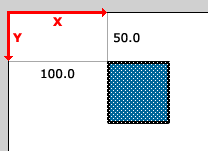
\includegraphics{wyznaczanie-pozycji-kursora}
\end{figure}

Uwzględniając różne proporcje \(p = \frac{szerokosc}{wysokosc}\) ekranu na którym pojawia się zdalnie sterowany kursor oraz proporcje powierzchni ekranu urządzenia mobilnego, w implementacji pilota użyta została reprezentacja procentowa punktu na ekranie.

Pozycja kursora reprezentowana jest przez punkt \(P(x, y)\) na dwuwymiarowej płaszczyźnie w zakresie \( x\in \langle0, 1\rangle \), gdzie \(x = \frac{x_{c}}{w_{x}}\), \(y = \frac{x_{c}}{w_{y}}\), a \(w_{x}\) oraz \(w_{y}\) oznaczają kolejno szerokość i wysokość ekranu.

Wyznaczanie pozycji uwzględnia również zmianę orientacji (poziomej lub pionowe), szerokości i wysokości rzutni okna przeglądarki wyświetlanej na urządzeniu mobilnym.

\lstset{language=JavaScript}
\begin{lstlisting}
this.run = function() {
	
	var this = that
	this.windowX = 0
	this.windowY = 0
	
	$(document).on('vmousemove', function(e) {
		e.preventDefault(); // prevent scroll
		
		var x = e.pageX / that.windowX
		var y = e.pageY / that.windowY
		
		console.log(x, y) // wypisz punkty
	})
	
	var indicateWindowSize = function() {
		that.windowX = $(window).width()
		that.windowY = $(window).height()
	}
	
	// register window size changes listeners
	$(window).on('resize orientationchange', function() {
		indicateWindowSize()
	})
	indicateWindowSize()
}
\end{lstlisting}

\subsection{Pamięć podręczna Web Storage}
